\section{Durchführung}
Zur Berechnung des Magnetfeldes der Spule wird eine Hall-Sonde verwendet.
Die Hall-Sonde beruht auf dem Hall-Effekt. An der Spitze der Hall-Sonde befindet sich
ein Leiterplättchen an das ein Strom angeschlossen ist. Durch ein Magnetfeld wirkt senkrecht
auf die Ladung die Lorenzkraft und erzeugt ein Verschiebungsstrom und ebenfalls eine Spannung (Hall-Spannung).
Mit Hilfe der Hall-Spannung kann die Stärke des Magnetfeldes, die von außen erzeugt worden ist, messen.
In Abbildung (\ref{abb:4}) ist der Versuchsaufbau dargestellt, dabei wird eine longitudinal Sonde verwenden.
Anschließend fährt die Sonde im Inneren der Magnetspule in verschiedenen Abstände ab und misst dabei das
Magnetfeld.
\begin{figure}[H]
  \centering
  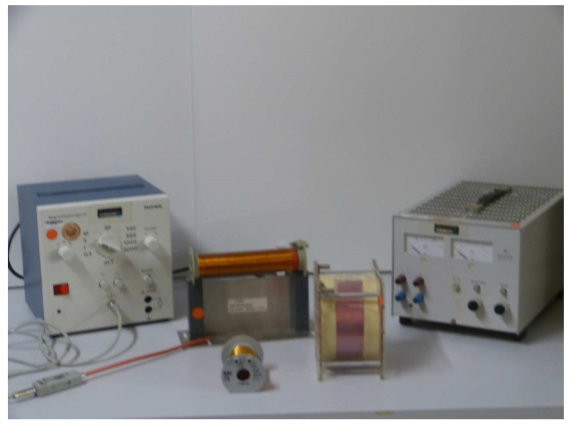
\includegraphics[width=10cm, height= 7cm]{Abb4.png}
  \caption{Versuchsaufbau zur Messung der Magnetspule[1].}
  \label{abb:4}
\end{figure}
Für die Messung des Magnetfeldes der Helmholz-Spule wird eine transversale Sonde verwendet.
Dabei wird im Inneren der beiden Spule als auch außerhalb die Magnetfelder gemessen.
In Abbildung (\ref{abb:5}) ist der Versuchsaufbau dargestellt.
\begin{figure}[H]
  \centering
  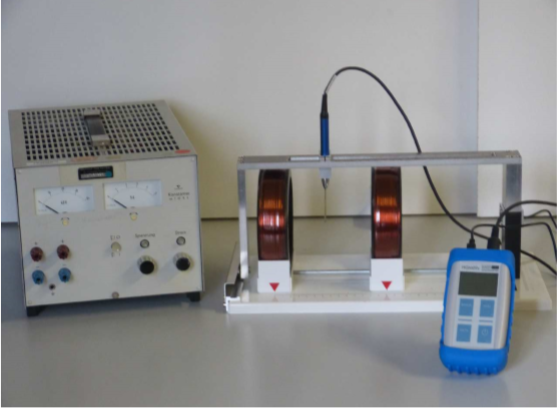
\includegraphics[width=10cm, height= 7cm]{Abb5.png}
  \caption{Versuchsaufbau zur Messung der Magnetfelder der Helmholz-Spule[1].}
  \label{abb:5}
\end{figure}
Für die Bestimmung der Hysteresekurve wird, wie in Abbildung(\ref{abb:6}) dargestellt,
ebenfalls eine transversale Sonde verwendet.
\begin{figure}[H]
  \centering
  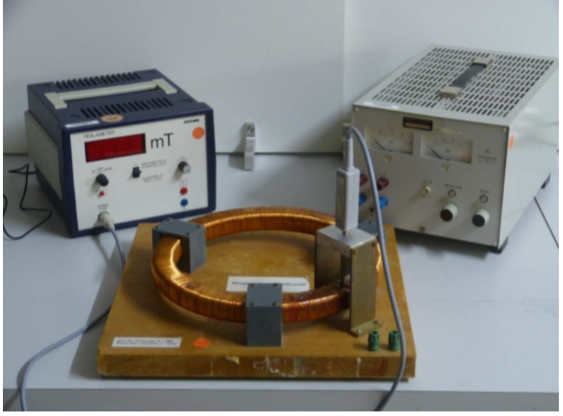
\includegraphics[width=10cm, height= 7cm]{Abb6.png}
  \caption{Versuchsaufbau zur Messung der Hysteresekurve[1].}
  \label{abb:6}
\end{figure}
